\newcommand{\titel}{Abschlussbericht ARM}
\title{\titel}
\newcommand{\untertitel}{uLoader WiSe 2014}
%\subtitle{\untertitel}
\newcommand{\autor}{Appel, Dennis (s813783)\\Voigt, Alexander (s814526)}
\author{\autor}
\date{\today}

\documentclass[
	11pt,				% Schriftgröße
	DIV10,
	german,				% für Umlaute, Silbentrennung etc.
	a4paper,			% Papierformat
	oneside,			% einseitiges Dokument
	titlepage,			% es wird eine Titelseite verwendet
	parskip=half,			% Abstand zwischen Absätzen (halbe Zeile)
	headings=normal,		% Größe der Überschriften verkleinern
	listof=totoc,			% Verzeichnisse im Inhaltsverzeichnis aufführen
	bibliography=totoc,		% Literaturverzeichnis im Inhaltsverzeichnis aufführen
	index=totoc,			% Index im Inhaltsverzeichnis aufführen
	captions=tableheading,		% Beschriftung von Tabellen unterhalb ausgeben
	final,				% Status des Dokuments (final/draft)
	numbers=endperiod
]{scrreprt}

\usepackage{scrhack}
\usepackage{yfonts}
% Zum Umfließen von Bildern -------------------------------------------------
\usepackage{floatflt}
\usepackage{lmodern}
\usepackage{textcomp}			% Euro-Zeichen etc.
\usepackage{listings}
\lstset{ %
	captionpos=b
}
\usepackage[ngerman]{babel}		% neue deutsche Rechtschreibung
\usepackage[utf8]{inputenc}
\usepackage[T1]{fontenc}
\usepackage{url}			% URL-Highlighting
\usepackage{amsmath,amsfonts}
% \usepackage{amsmath}
%\usepackage{times}
\usepackage{setspace}
\usepackage{multirow}
%\usepackage{amsfonts}
%\usepackage{amssymb}
\usepackage{array}
\usepackage[
	automark,			% Kapitelangaben in Kopfzeile automatisch erstellen
	headsepline,			% Trennlinie unter Kopfzeile
	ilines				% Trennlinie linksbündig ausrichten
]{scrpage2}
\usepackage[labelfont=bf, belowskip=4pt, hypcap]{caption}
\usepackage{a4wide}
%\usepackage{mathrsfs}
%\usepackage{mathtools}
\usepackage{graphicx}
%\usepackage{wasysym}
%\usepackage{pgfplots}
\usepackage{cite}
% Text um Bilder fliessen lassen
\usepackage{wrapfig}
\usepackage{float}
\usepackage{pdfpages}
\usepackage{geometry}
% \geometry{paper=a4paper,left=35mm,right=35mm,top=30mm}
\usepackage[square]{natbib}
\usepackage{tikz}
\usetikzlibrary{arrows,shapes,positioning,shadows,trees}

\tikzset{
  basic/.style  = {draw, text width=2cm, drop shadow, font=\sffamily, rectangle},
  root/.style   = {basic, rounded corners=2pt, thin, align=center,
                   fill=green!30},
  level 2/.style = {basic, rounded corners=6pt, thin,align=center, fill=green!60,
                   text width=8em},
  level 3/.style = {basic, thin, align=left, fill=pink!60, text width=8em}
}

% Kopf- und Fußzeilen
\pagestyle{scrheadings}

% Kopf- und Fußzeile auch auf Kapitelanfangsseiten
\renewcommand*{\chapterpagestyle}{scrheadings}

% Schriftform der Kopfzeile
\renewcommand{\headfont}{
	\normalfont
}

% Kopfzeile
\ihead{\large{\textsc{\titel}}\\ \textit{\headmark}}
\chead{}
\ohead{} %\vspace{0.5cm} \includegraphics[scale=0.3]{Beuth_Logo_horizontal}}
%
\setlength{\headheight}{21mm}		% Höhe der Kopfzeile
\setlength{\parindent}{5mm}		% Einzug bei neuem Absatz
\setheadwidth[0pt]{textwithmarginpar}	% Kopfzeile über den Text hinaus verbreitern
\setheadsepline[text]{0.4pt}		% Trennlinie unter Kopfzeile

% Fußzeile
\ifoot{}
\cfoot{\textsc{\footnotesize{\untertitel}}}
\ofoot{\pagemark}

\subtitle{\untertitel}

% erzeugt ein wenig mehr Platz hinter einem Punkt
\frenchspacing

% Schusterjungen und Hurenkinder vermeiden
\clubpenalty		= 10000
\widowpenalty		= 10000
\displaywidowpenalty	= 10000

% mach pdf searchable
\usepackage{lmodern}
\input{glyphtounicode}
\pdfgentounicode=1

% \usepackage[bookmarks,bookmarksnumbered]{hyperref}
\usepackage[
bookmarks,
bookmarksopen=true,
pdftitle={\titel},
% pdfauthor={\autor},
% pdfcreator={\autor},
pdfsubject={\titel},
pdfkeywords={\titel},
colorlinks=true,
linkcolor=red, % einfache interne Verknüpfungen
anchorcolor=black,% Ankertext
citecolor=blue, % Verweise auf Literaturverzeichniseinträge im Text
filecolor=magenta, % Verknüpfungen, die lokale Dateien öffnen
menucolor=red, % Acrobat-Menüpunkte
urlcolor=cyan,
% linkcolor=black, % einfache interne Verknüpfungen
% anchorcolor=black,% Ankertext
% citecolor=black, % Verweise auf Literaturverzeichniseinträge im Text
% filecolor=black, % Verknüpfungen, die lokale Dateien öffnen
% menucolor=black, % Acrobat-Menüpunkte
% urlcolor=black,
backref,
%pagebackref,
plainpages=false,% zur korrekten Erstellung der Bookmarks
pdfpagelabels,% zur korrekten Erstellung der Bookmarks
hypertexnames=false,% zur korrekten Erstellung der Bookmarks
% linktocpage, % Seitenzahlen anstatt Text im Inhaltsverzeichnis verlinken
% linkcolor=red % Linkfarbe f\"ur den Druck auf schwarz, f\"ur die PDF-Version auf rot stellen
]{hyperref}

\setcounter{secnumdepth}{5}
\setcounter{tocdepth}{5}
\newcommand*{\fullref}[1]{\hyperref[{#1}]{\autoref*{#1} \nameref*{#1}}}

\makeindex

\begin{document}
\maketitle
\pagenumbering{Roman}
\tableofcontents
\listoffigures					% Abbildungsverzeichnis
\listoftables					% Tabellenverzeichnis
\lstlistoflistings
\clearpage
\pagenumbering{arabic}
\chapter{Introduction}
 
Nowadays, an ARM-MCU could be used in every aspect of everyday life.
Additionally, the ARM processor is the number one architecture of choice in 
many market segments.\\\\ 
This project is based on the development of a bootloaders and its implementation 
inside a network. The usage stm32f4-discovery Board is a prefered and viewed as an 
"'Allrounder"' for such a project. The reasoning behind this is the "value for money" 
and user-friendliness. This allows for an easy introduction into the world of ARM
Microcontroller unit programming.\\
The ARM-Cortex-M4-Prozessor found on the STM32f4-discovery board processes 
the principel parts shown in the figure below.\\
The aim of the project is to research the feasibility to create a quick, cheap 
and easy to use way of utilizing an STM32 Microcontroller to communicate between 
a user and a remote device.\\\\
The purpose of the application is meant to be a first step fundamental strategy to 
creating a product for future projects.\\
It is hoped that by utilizing a boot loader, a fast and light application could 
be used to fulfill the desire of a user to achieve a particular objective such 
as, threeway handshake signal to verify a particular device in order to transmit 
information such as codes or messages, using a TCP/IP protocol stake.\\
As it can be demonstrated the different applications could be endless.\\ 

\begin{figure}[ht]
	\centering
	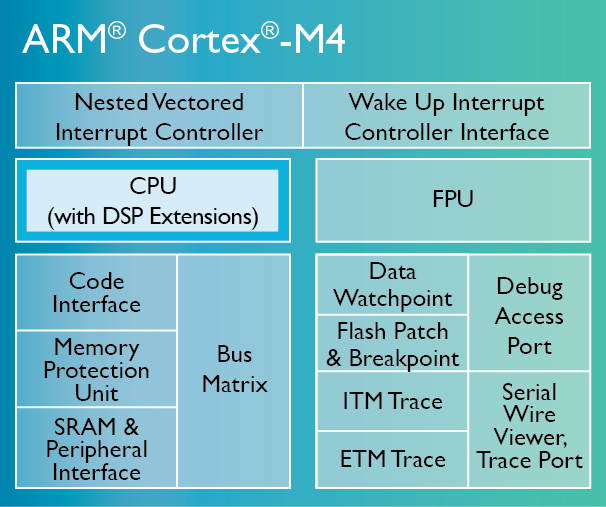
\includegraphics[width=400px, height=300px]{../img/Cortex-M4-chip-diagram-LG.png}
	\caption{Prinzipieller Aufbau}
	\label{m4_prinzip}
\end{figure}

Analogously, a new and different diagram would be used, in order to illustrate the 
change in the usage-concept of the processors.\\

But first, an overview of the discussed focal points would be outlined.\\  


\section{Bootloader}
The purpose of a Bootloader program is to allow the installation and utilisation 
of any program that could be reloaded. Whereas the program that is currently loaded is also being run.\\
Next it is necessary to initialise the hardware, that would in turn be needed to load the program.\\
The "STM32f407 discovery board" offers three different methodes to boot up the hardware.\\
In order to switch between the three different boot methods, the Boot-Pins BOOT1
and BOOT2 could be set:
\begin{table}[ht]
\centering
\begin{tabular}{|c|c|l|l|}
\hline \hline
  BOOT1 & BOOT2 & Boot-Mode & Adresse\\ \hline
  x & 0 & Flash Memory (User Flash) & 0x8000\_0000\\
\hline
  0 & 1 & System Memory & 0x1FFF\_F000\\
\hline
 1  & 1 & SRAM & 0x2000\_0000\\
\hline
\end{tabular}
\caption{Boot-Pin Function}
\end{table}\\\\

The ROM memory is included by the manufacturer along with the bootloader.\\
It is very important to set the correct address of the program, that is located 
in the memory, in order for the reloading of the program to work.\\
A step by step example of the the sequence after the boot loader is already 
loaded , is as follows:

\begin{enumerate}
\item Hardware initialize (USB / USART / RCC ... )
\item Wait for running program (pending other tasks)
\item Write a program to address XY.
\item Point to address XY
\end{enumerate}

After these steps, the newly setup program is then responsible for the initialization 
of the hardware.\\

\section{SWD}
During the development of the Boot Loader, a serial wire debug technology was used. 
The reason behind this is to utilize a Debug-Port that has been specially developed to 
cater to a MCU that makes allows the use of the least amount of pins possible.\\
This port consists of pins shown in the following:\\
\begin{table}[ht]
\centering
\begin{tabular}{|c|c|c|p{10cm}|}
\hline \hline
	Pin & Signal & Type & Description \\ \hline
1 & VTref & Input & This is the target reference voltage. It is used to
 check if the target has power, to create the logic-level reference for
 the input comparators and to control the output logic levels to the target.
 It is normally fed from Vdd of the target board and must not have a series resistor.\\ \hline
7 & SWDIO & I/O & Single bi-directional data pin\\ \hline
9 & SWCLK & Output & Clock signal to target CPU. It is recommended that
 this pin is pulled to a defined state of the target board. Typically
 connected to TCK of target CPU.\\ \hline
13 & SWO & Output & Serial Wire Output trace port. (Optional, not required
for SWD communication)\\ \hline
15 & RESET & I/O & Target CPU reset signal. Typically connected to the
 RESET pin of the target CPU, which is typically called "nRST", "nRESET"
 or "RESET".\\ \hline
19 & 5V-Supply & Output & This pin is used to supply power to some eval boards.
Not all JLinks supply power on this pin, only the KS (Kickstart) versions.
Typically left open on target hardware.\\ \hline
\end{tabular}
\caption{SWD PINOUT}
\end{table}\\

The other pins of the 20-pole connection are going to left out, meaning, the other 
pins are useless for the SWD or they will be used as a GND. Regardless of the pin allocation, 
it is important that the communication of the SWD would not be interrupted or effected. 

This technique represents a new and more effective way to debuggen. Until now JTAG 
represented the Debugger-Interface.  


The advantages of this technology are:

\begin{itemize}
\item Only 2 Pins are used
\item JTAG TAP controller compatible
\item Allows the Debugger to become an extra AMBA-Bus-Master, in order to accomidate an extra 
access capability to the Register or Memory
\item High Datarates - 4Mbytes/sec @50MHz
\item Low Power - no extra power supply 
\item Error recognition "'built in"' that performs well
\item Protection against errors that cause disconnection
\end{itemize}  

\section{Startup}
 - stack, program counter, interrupt, vector table, initial system clock

\section{CMSIS}
The ARM Cortex Microcontroller Software Interface Standard is a manufacturer independent 
abstraction layer for the Cortex-M processors.\\
Thereby the CMSIS is subdivided into:
\begin{itemize}
\item CMSIS-CORE - API access to the processor kernal and peripheral register.
\item CMSIS-Driver - Generic access on peripheral devices for Middleware
			(reusability).
\item CMSIS-DSP - DSP Liberary with over 60 functions
\item CMSIS-RTOS API - Standardised (RTOS compatible)
\item CMSIS-Pack - Description of the most important components (User view)
\item CMSIS-SVD - Description of the most important components (System view)
\item CMSIS-DAP - Debug Access Port
\end{itemize}

Summarized, CMSIS allows a consistent and simple software interfaced to the processor 
and peripheral devices, as well as Real-time OS (RTOS) and Middleware.

\section{Nested Vectored Interrupt Controller}
The NVIC offers the possibility to configure special interrupts 
(Priority, Activate, Deactivate...). \\
Aside from the given interrupts, there are also the configurable implementation dependent interrupts.  
Because, the first 15 interrupts are allocated, the number of implimented interrupts could be from 0-240.

\section{Differences }
GNU, KEIL iar

\section{Network}
was sollte zum besseren verstehen hier einen platz finden.

\chapter{Einleitung}

Es gibt nahezu keinen Bereich, indem ARM-MCU heutzutage keine Verwendung finden. 
Zudem gilt ARM als f\"uhrende Architektur in vielen Marktsegementen.\\ 
Das Projekt beinhaltet die Entwicklung eines Bootloaders sowie die
 Netzwerkimplementierung.\\
Das verwendete stm32f4-discovery Board ist ein beliebter "'Allrounder"'.
Die Begr\"undung daf\"ur ist das Preis-Leistungs-Verh\"altnis und die
Benutzerfreundlichkeit. Diese erlaubt einen leichten Um- bzw. Einstieg in
die ARM-MCU-Programmierung.\\
Der auf dem Board verwendete ARM-Cortex-M4-Prozessor beinhaltet (Prinzip)
Bestandteile der folgenden Grafik entsprechend.\\
\begin{figure}[ht]
	\centering
	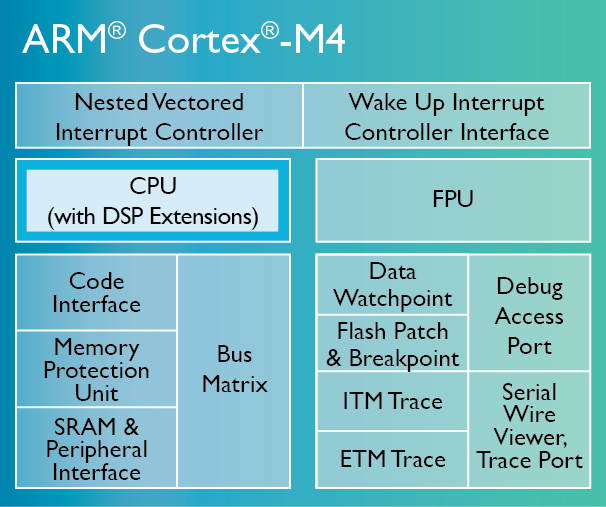
\includegraphics[width=400px, height=300px]{../img/Cortex-M4-chip-diagram-LG.png}
	\caption{Prinzipieller Aufbau}
	\label{m4_prinzip}
\end{figure}

Es wird sp\"ater ein weiteres unterschiedliches Diagram verwendet. Dies ist nicht
falsch, sondern dient der sinngem\"a"sen Darstellung des Prozessors.\\

Zun\"achst soll ein \"Uberblick \"ueber die behandelten Themenschwerpunkte gegeben
 werden

\section{Bootloader}
Ein Booloader ist ein Programm, welches es erm\"oglicht ein beliebiges weiteres
 Programm nachzuladen. Wobei das nachzuladene Programm das Eigentliche ist, 
welches ausgef\"uhrt werden soll.\\
Dazu ist es notwendig die Hardware zu initialisieren, die ben\"otigt wird um das
 eigentliche Programm mit der gew\"ahlten Methode nachzuladen.\\
Das stm32f407 discovery board bietet drei verschiedene Arten an um zu booten.\\
Um zwischen den drei Varianten w\"ahlen zu k\"onnen, sind die Boot-Pins BOOT1
und BOOT2 entsprechend zu setzen:\\\\
\begin{tabular}{|c|c|l|l|}
\hline \hline
  BOOT1 & BOOT2 & Boot-Mode & Adresse\\ \hline
  x & 0 & Flash Memory (User Flash) & 0x8000\_0000\\
\hline
  0 & 1 & System Memory & 0x1FFF\_F000\\
\hline
 1  & 1 & SRAM & 0x2000\_0000\\
\hline
\end{tabular}\\\\
Der ROM, hier System Memory, beinhaltet den, vom Hersteller, mitgegebenen
 Bootloader.\\
Wie man den Speicher dann belegt ist einem freigestellt. Man muss dann darauf
achten, dass man an die richtige Adresse springt, wenn man das Programm nachgeladen
hat.\\
Als Beispiel-Vorgehensweise kann man sagen, dass die Reihenfolge, nachdem der
Bootloader bereits geladen ist, folgende ist:\\

\begin{enumerate}
\item Verwendete Hardware initialisieren (USB/USART/RCC...)
\item Auf eingehendes Programm warten (wenn sonst keine Aufgabe ansteht)
\item Eingehendes Programm an Adresse XY schreiben.
\item An Adresse XY springen
\end{enumerate}

Das eingegangene Programm ist dann nat\"urlich selbst f\"ur die Initialisierung
der verwendeten Hardware zust\"andig.\\

\section{SWD}
Bei der Entwicklung kam die Serial Wire Debug Technologie zum Einsatz. Hierbei 
handelt es sich um einen Debug-Port, der speziell daf\"ur entwickelt wurde
 um MCU bzw. Projekte mit MCU, bei denen so wenig wie m\"oglich Pins verwendet
 werden sollen. \\
Dieser Port besteht aus den Leitungen folgender Tabelle:\\\\
\begin{tabular}{|c|c|c|p{10cm}|}
\hline \hline
	Pin & Signal & Type & Beschreibung \\ \hline
1 & VTref & Input & This is the target reference voltage. It is used to
 check if the target has power, to create the logic-level reference for
 the input comparators and to control the output logic levels to the target.
 It is normally fed from Vdd of the target board and must not have a series resistor.\\ \hline
7 & SWDIO & I/O & Single bi-directional data pin\\ \hline
9 & SWCLK & Output & Clock signal to target CPU. It is recommended that
 this pin is pulled to a defined state of the target board. Typically
 connected to TCK of target CPU.\\ \hline
13 & SWO & Output & Serial Wire Output trace port. (Optional, not required
for SWD communication)\\ \hline
15 & RESET & I/O & Target CPU reset signal. Typically connected to the
 RESET pin of the target CPU, which is typically called "nRST", "nRESET"
 or "RESET".\\ \hline
19 & 5V-Supply & Output & This pin is used to supply power to some eval boards.
Not all JLinks supply power on this pin, only the KS (Kickstart) versions.
Typically left open on target hardware.\\ \hline
\end{tabular}\\\\

Die anderen Leitungen des bisherigen 20-poligen Anschlussen wurden weggelassen,
weil sie entweder f\"ur SWD uinteressant sind oder sie auf GND gelegt sind. Egal
was davon zutrifft, sie haben keinen Einfluss auf die SWD-Kommunikation.

Es ist eine neue, sehr interessante Weise zu debuggen. Bisher war JTAG das
Debugger-Interface. 
Die Vorteile dieser Technologie sind (frei von der ARM-Website \"ubersetzt):

\begin{itemize}
\item Nur 2 Pins werden belegt
\item JTAG TAP controller kompatibel
\item Erlaubt dem Debugger ein weiterer AMBA-Bus-Master zu werden um auf
Register / Speicher zuzugreifen.
\item High Datarates - 4Mbytes/sec @50MHz
\item Low Power - keine zus\"atzlichen Versorgungsspannung
\item gute "'built in"' Fehler-Erkennung
\item Schutz vor Fehlern bei Kontaktverlust
\end{itemize}  

\section{startup}
 - stack, program counter, interrupt, vector table, initial system clock

\section{CMSIS}
Der ARM Cortex Microcontroller Software Interface Standard ist eine 
H\"andlerunabh\"angige Abstraktionsschicht f\"ur die Cortex-M Prozessoren.\\
Dabei ist CMSIS unterteilt in:
\begin{itemize}
\item CMSIS-CORE - API zum Zugriff auf den Prozessorkern sowie Perepherie-Register.
\item CMSIS-Driver - Generischer Zugriff auf Perepherie f\"ur die Middleware
			(reusability).
\item CMSIS-DSP - DSP Bibliothek mit \"uber 60 Funktionen
\item CMSIS-RTOS API - Standardisiertes (RTOS kompatibel)
\item CMSIS-Pack - Beschreibung der wichtigen Bestandteile (Nutzersicht)
\item CMSIS-SVD - Beschreibung der wichtigen Bestandteile (Systemsicht)
\item CMSIS-DAP - Debug Access Port
\end{itemize}

Zusammengefasst erlaubt CMSIS einheitliche und simple Software Schnittstelle
zu Prozessor und die Perepherie, sowie Echtzeit OS (RTOS) und Middleware.

\chapter{Nested Vectored Interrupt Controller}
Der NVIC bietet die M\"oglichkeit gewisse Interrupts zu konfigurieren
(Priorit\"at, aktiviert, deaktiviert...). \\
Neben vorgegebenen Interrupts sind hier auch die Implementierungsabh\"angigen
Interrupts konfigurierbar. Da die ersten 15 Interrupts vorgegeben sind, k\"onnen
die implementierten Interrupts in der Anzahl von 0 bis 240 reichen.

\section{Unterschiede}
GNU, KEIL iar

\section{Netzwerk}
was sollte zum besseren verstehen hier einen platz finden.



\bibliography{Bibliographie}			% Aufruf: bibtex FHWTVorlage
\bibliographystyle{natdin}			% DIN-Stil des Literaturverzeichnisses
% Anhang -------------------------------------------------------------------
%		Die Inhalte des Anhangs werden analog zu den Kapiteln inkludiert.
%		Dies geschieht in der Datei Anhang.tex
% --------------------------------------------------------------------------
% \begin{appendix}
% 	\clearpage
% 	\pagenumbering{roman}
% 	\input{appendix}
% \end{appendix}
\end{document}
